% !TeX spellcheck = en_GB
% /*
%  * ----------------------------------------------------------------------------
%  * "THE BEER-WARE LICENSE" (Revision 42):
%  * <michi.wieland@hotmail.com> wrote this file. As long as you retain this notice you
%  * can do whatever you want with this stuff. If we meet some day, and you think
%  * this stuff is worth it, you can buy me a beer in return. Michael Wieland
%  * ----------------------------------------------------------------------------
%  */

\documentclass[
a4paper,
oneside,
10pt,
fleqn,
headsepline,
toc=listofnumbered, 
bibliography=totocnumbered]{scrartcl}

% deutsche Trennmuster etc.
\usepackage[T1]{fontenc}
\usepackage[utf8]{inputenc}
\usepackage[english, ngerman]{babel} % \selectlanguage{english} if  needed
\usepackage{lmodern} % use modern latin fonts

% Custom commands
\newcommand{\AUTHOR}{Fabian Hauser \& Muriele Trentini}
\newcommand{\INSTITUTE}{Hochschule für Technik Rapperswil}
\newcommand{\GITHUB}{https://github.com/michiwieland/hsr-zusammenfassungen}
\newcommand{\LICENSEURL}{https://en.wikipedia.org/wiki/Beerware}
\newcommand{\LICENSE}{
"THE BEER-WARE LICENSE" (Revision 42):
<michi.wieland@hotmail.com> wrote this file. As long as you retain this notice you
can do whatever you want with this stuff. If we meet some day, and you think
this stuff is worth it, you can buy me a beer in return. Michael Wieland	
}

% Jede Überschrift 1 auf neuer Seite
\let\stdsection\section
\renewcommand\section{\clearpage\stdsection}

% Multiple Authors
\usepackage{authblk}

% Layout / Seitenränder
\usepackage{geometry}

% Inhaltsverzeichnis
\usepackage{makeidx} 
\makeindex

\usepackage{url}
\usepackage[pdfborder={0 0 0}]{hyperref}
\usepackage[all]{hypcap}
\usepackage{hyperxmp} % for license metadata

% Glossar und Abkürzungsverzeichnis
\usepackage[acronym,toc,nopostdot]{glossaries}
\glossarystyle{altlisthypergroup}
\usepackage{xparse}
\DeclareDocumentCommand{\newdualentry}{ O{} O{} m m m m } {
	\newglossaryentry{gls-#3}{name={#5},text={#5\glsadd{#3}},
		description={#6},#1
	}
	\makeglossaries
	\newacronym[see={[Siehe:]{gls-#3}},#2]{#3}{#4}{#5\glsadd{gls-#3}}
}
\makeglossaries

% Mathematik
\usepackage{amsmath}
\usepackage{amssymb}
\usepackage{amsfonts}
\usepackage{enumitem}

% Images
\usepackage{graphicx}
\graphicspath{{images/}} % default paths

% Boxes
\usepackage{fancybox}

%Tables
\usepackage{tabu}
\usepackage{booktabs} % toprule, midrule, bottomrule
\usepackage{array} % for matrix tables

% Multi Columns
\usepackage{multicol}

% Header and footer
\usepackage{scrlayer-scrpage}
\setkomafont{pagehead}{\normalfont}
\setkomafont{pagefoot}{\normalfont}
\automark*{section}
\clearpairofpagestyles
\ihead{\headmark}
\ohead{\AUTHOR}
\cfoot{\pagemark}

% Pseudocode
\usepackage{algorithm}
\usepackage{algorithmic}

% Code Listings
\usepackage{listings}
\usepackage{color}
\usepackage{beramono}

\definecolor{DarkPurple}{rgb}{0.4, 0.1, 0.4}
\definecolor{DarkCyan}{rgb}{0.0, 0.5, 0.4}
\definecolor{LightLime}{rgb}{0.3, 0.5, 0.4}
\definecolor{Blue}{rgb}{0.0, 0.0, 1.0}

\lstdefinestyle{eclipse-style}{
	language=Java,  
	columns=flexible,
	showstringspaces=false,     
	basicstyle=\footnotesize\ttfamily, 
	keywordstyle=\bfseries\color{DarkPurple},
	commentstyle=\color{LightLime},
	stringstyle=\color{Blue}, 
	escapeinside={£}{£}, % latex scope within code      
	morekeywords={length},
	numbers=left,
	numberstyle=\tiny\color{black},
	frame=single,
}
\lstset{style=eclipse-style}


% Theorems \begin{mytheo}{title}{label}
\usepackage{tcolorbox}
\tcbuselibrary{theorems}
\newtcbtheorem[number within=section]{definiton}{Definition}%
{fonttitle=\bfseries}{def}
\newtcbtheorem[number within=section]{remember}{Merke}%
{fonttitle=\bfseries}{rem}

% Dokumentinformationen
\newcommand{\SUBJECT}{Zusammenfassung}
\newcommand{\TITLE}{Programmieren und Formale Methoden}

\loadglsentries{glossar}

% pdf metadata
\hypersetup{
	pdfauthor={\AUTHOR},
	pdftitle={\SUBJECT \TITLE},
	pdfcopyright={\LICENSE},
	pdflicenseurl={\LICENSEURL}
}

\begin{document}
	
% Front page
\title{\TITLE}
\subject{\SUBJECT}
\author{\AUTHOR}
\affil{\INSTITUTE}
\date{\today}
\maketitle

\vfill

% Participate
\paragraph{Mitmachen} \hfill \\
Falls Du an diesem Dokument mitarbeiten willst, kannst Du das Dokument
auf GitHub unter \url{\GITHUB} forken.

% Licence
\paragraph{Lizenz} \hfill \\
\LICENSE

% Table of contents
\tableofcontents


% Glossar and acronyms (if included \loadglsentries{glossar})
\printglossary[type=\acronymtype]
\printglossary
\glsaddall


\section{Introduction}
The use of a formal language is to describe and solve problems is central to computer science.

\begin{description}
	\item[Formal Methods] Make computer programming more reliable and predictable by mathematical analysis.
	\item[Formal Language] Set of string of symbols that are constrained by specific rules. Membership in this set can automatically be determined (mechanical processing possible)
	\item[Informal Language] Any living natural language
\end{description}

\section{Programming Paradigms}

Paradigm is a Worldview / Concept / Tought patterns.

OOP uses multiple of the paradigms below, but is not a paradigm in this sense.

\subsection{The Imperative Programming Paradigm}

Is imperative (de: Befehlend) and focuses on \emph{how} a program works, like a recipee. It uses commands to change the program's state.

A program (in this course) is a sequence of commands and the computation is a change of state.

Most hardware implementations of computer is imperative.

It is based on the Von Neumann architecture.

\subsubsection{Basic Building Blocks}

\begin{description}
	\item[Assignments (sate/store/heap)] x:= x+1 %TODO: COde
	\item[Sequential composition] ...; ...
	\item[Conditional excetion] if ... then ... else...
	\item[Repetition] while .. do .. / goto ...
\end{description}



\subsection{The Declarative Programming Paradigm}

Discribe logic of computation without expicitly describing its control flow.

\emph{What} should a programm accomplish, not how the language should do smth. (But it must still be computable in the end).

Programs are here theories of a formal logic. Computations are deductions.

Examples: Spreadsheets, Regex, Query Languages (SQL etc.), Functional programming languages (Haskel, ...), Logic programming (Prolog)

\subsubsection{The Functional Programming Paradigm}

Basis: The Lambda Calculus

Programs are function definitions, computations are function evaluations.

\subsubsection{The Logical Programming Paradigm}
Basis: Predicate logic

Programs are rules in predicate logic and computation is a proof of a predicate.



\section{Formal Proof (Propositional and Predicate logic)}

\begin{figure}
	\centering
	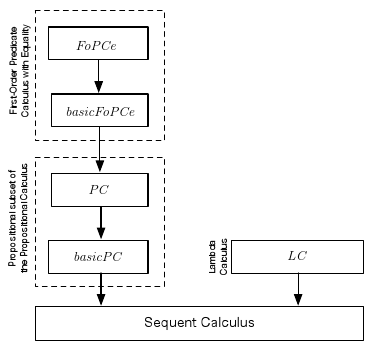
\includegraphics[width=0.7\linewidth]{images/sequent_calculus_overview}
	\caption{Overview calculus proof family.}
	\label{fig:sequentcalculusoverview}
\end{figure}

\subsection{refresher ''Diskrete Mathematik''}
Kinds of logic: Boolean, ''Prädikatenlogik'' ($\forall,\exists, \Rightarrow, \Leftrightarrow, \wedge, \vee, \neg$)

Proofs: induction, direct, indirect, by contradiction

\subsection{What are formal and informal proofs?}
A \emph{informal proof} are arguments presented as explanations in natural language (like most mathematical textbooks; need a human to check)

A \emph{formal proof} is constructed using well-formed formulas of a formal language and formally defined rules of inference.
 They can be checked by a machine and sometimes be mechanically constructed. Computer programs are able to assist proving (e.g. like Excel), sometimes a proof is even not practically possible without them.

\subsection{Sequent Calculus style}

Most programming languages are defined in the sequence calculus style; often used for types and programming languages, semantics and proofs of languages.


\subsubsection{Proof Rules}

 A device to construct proofs.
 
 \[
 \frac{\overrightarrow{A}}{C} \boldmath{r}
 \]
 
 \begin{description}
	 	\item[$r$] Rule name
	 	\item[$C$] Consequent (to be proven)
	 	\item[$\vec{A}$] list of sequent proof rules (vector).
 	\end{description}
 	
 
 We want to proof $C$ out of multiple sequent proof rules $A_1, A_2, ..., A_n$ with the rule $r$. If there is no $A$ above the line, the proof rule is a axiom. The order of proof rules $A$ is important and not permutable.
 
 To build a complete proof, all proof rules must be proven up to a axiom.


\subsubsection{Definitions}

\begin{description}
	\item[Sequent] a proof rule or axiom
	\item[Proof Rule] A rule $r$ to proof a consequent $C$ with more proof rules $A$
	\item[pending sub-goal] A sequent which is not yet proven by a axiom.
	\item[Axiom] Proof rule without sequent $A$; assumed to be true. \\
	There should be as less as possible axioms.
	\item[Calculus (or Theory)] (possibly infinite) set of proof rules $r_1$, $r_2$.
	\item[Proof (or Derivations)] Ordered proof rules in a tree, so that all proof rules are proven by a axiom.
\end{description}

\subsubsection{Example}

\paragraph{Type checking proof}

of the shorthand if else construct for integers.

\[
	\frac{
			\frac{
				\frac{}{x::int}x_{int} \text{   } \frac{}{y::int}y_{int}
			}{(x > y)::bool} \text{   }
		  \frac{
				\frac{}{x::int}x_{int} \text{   } \frac{}{y::int}y_{int}
			}{(x - y)::int} -_{int1} \text{   }
			\frac{
				\frac{}{y::int}y_{int} \text{   } \frac{}{x::int}x_{int}
			}{(y - x)::int} -_{int2}
		}{(x>y? x - y : y - x)::int} condExpr_{int}
\]

\subsection{Propositional Calculus}


\section{Logic programming (Prolog)}

\section{Lambda calculus}

\section{Functional Programming (Haskell)}

\section{Multi-Paradigm Programming (Scala)}


\appendix

% Code Listings
\lstlistoflistings

% List of figures
\listoffigures

% List of tables
\listoftables

% Bibliography
\bibliographystyle{plain} 
\bibliography{literatur}

\end{document}
